\section{System Architecture and Candidate Blackboard}
\label{sec:system_architecture}
Fig.~\ref{fig:arch} illustrates the modular architecture of ROUTE/IQ-NextGen.

\begin{figure*}[t]
\centering
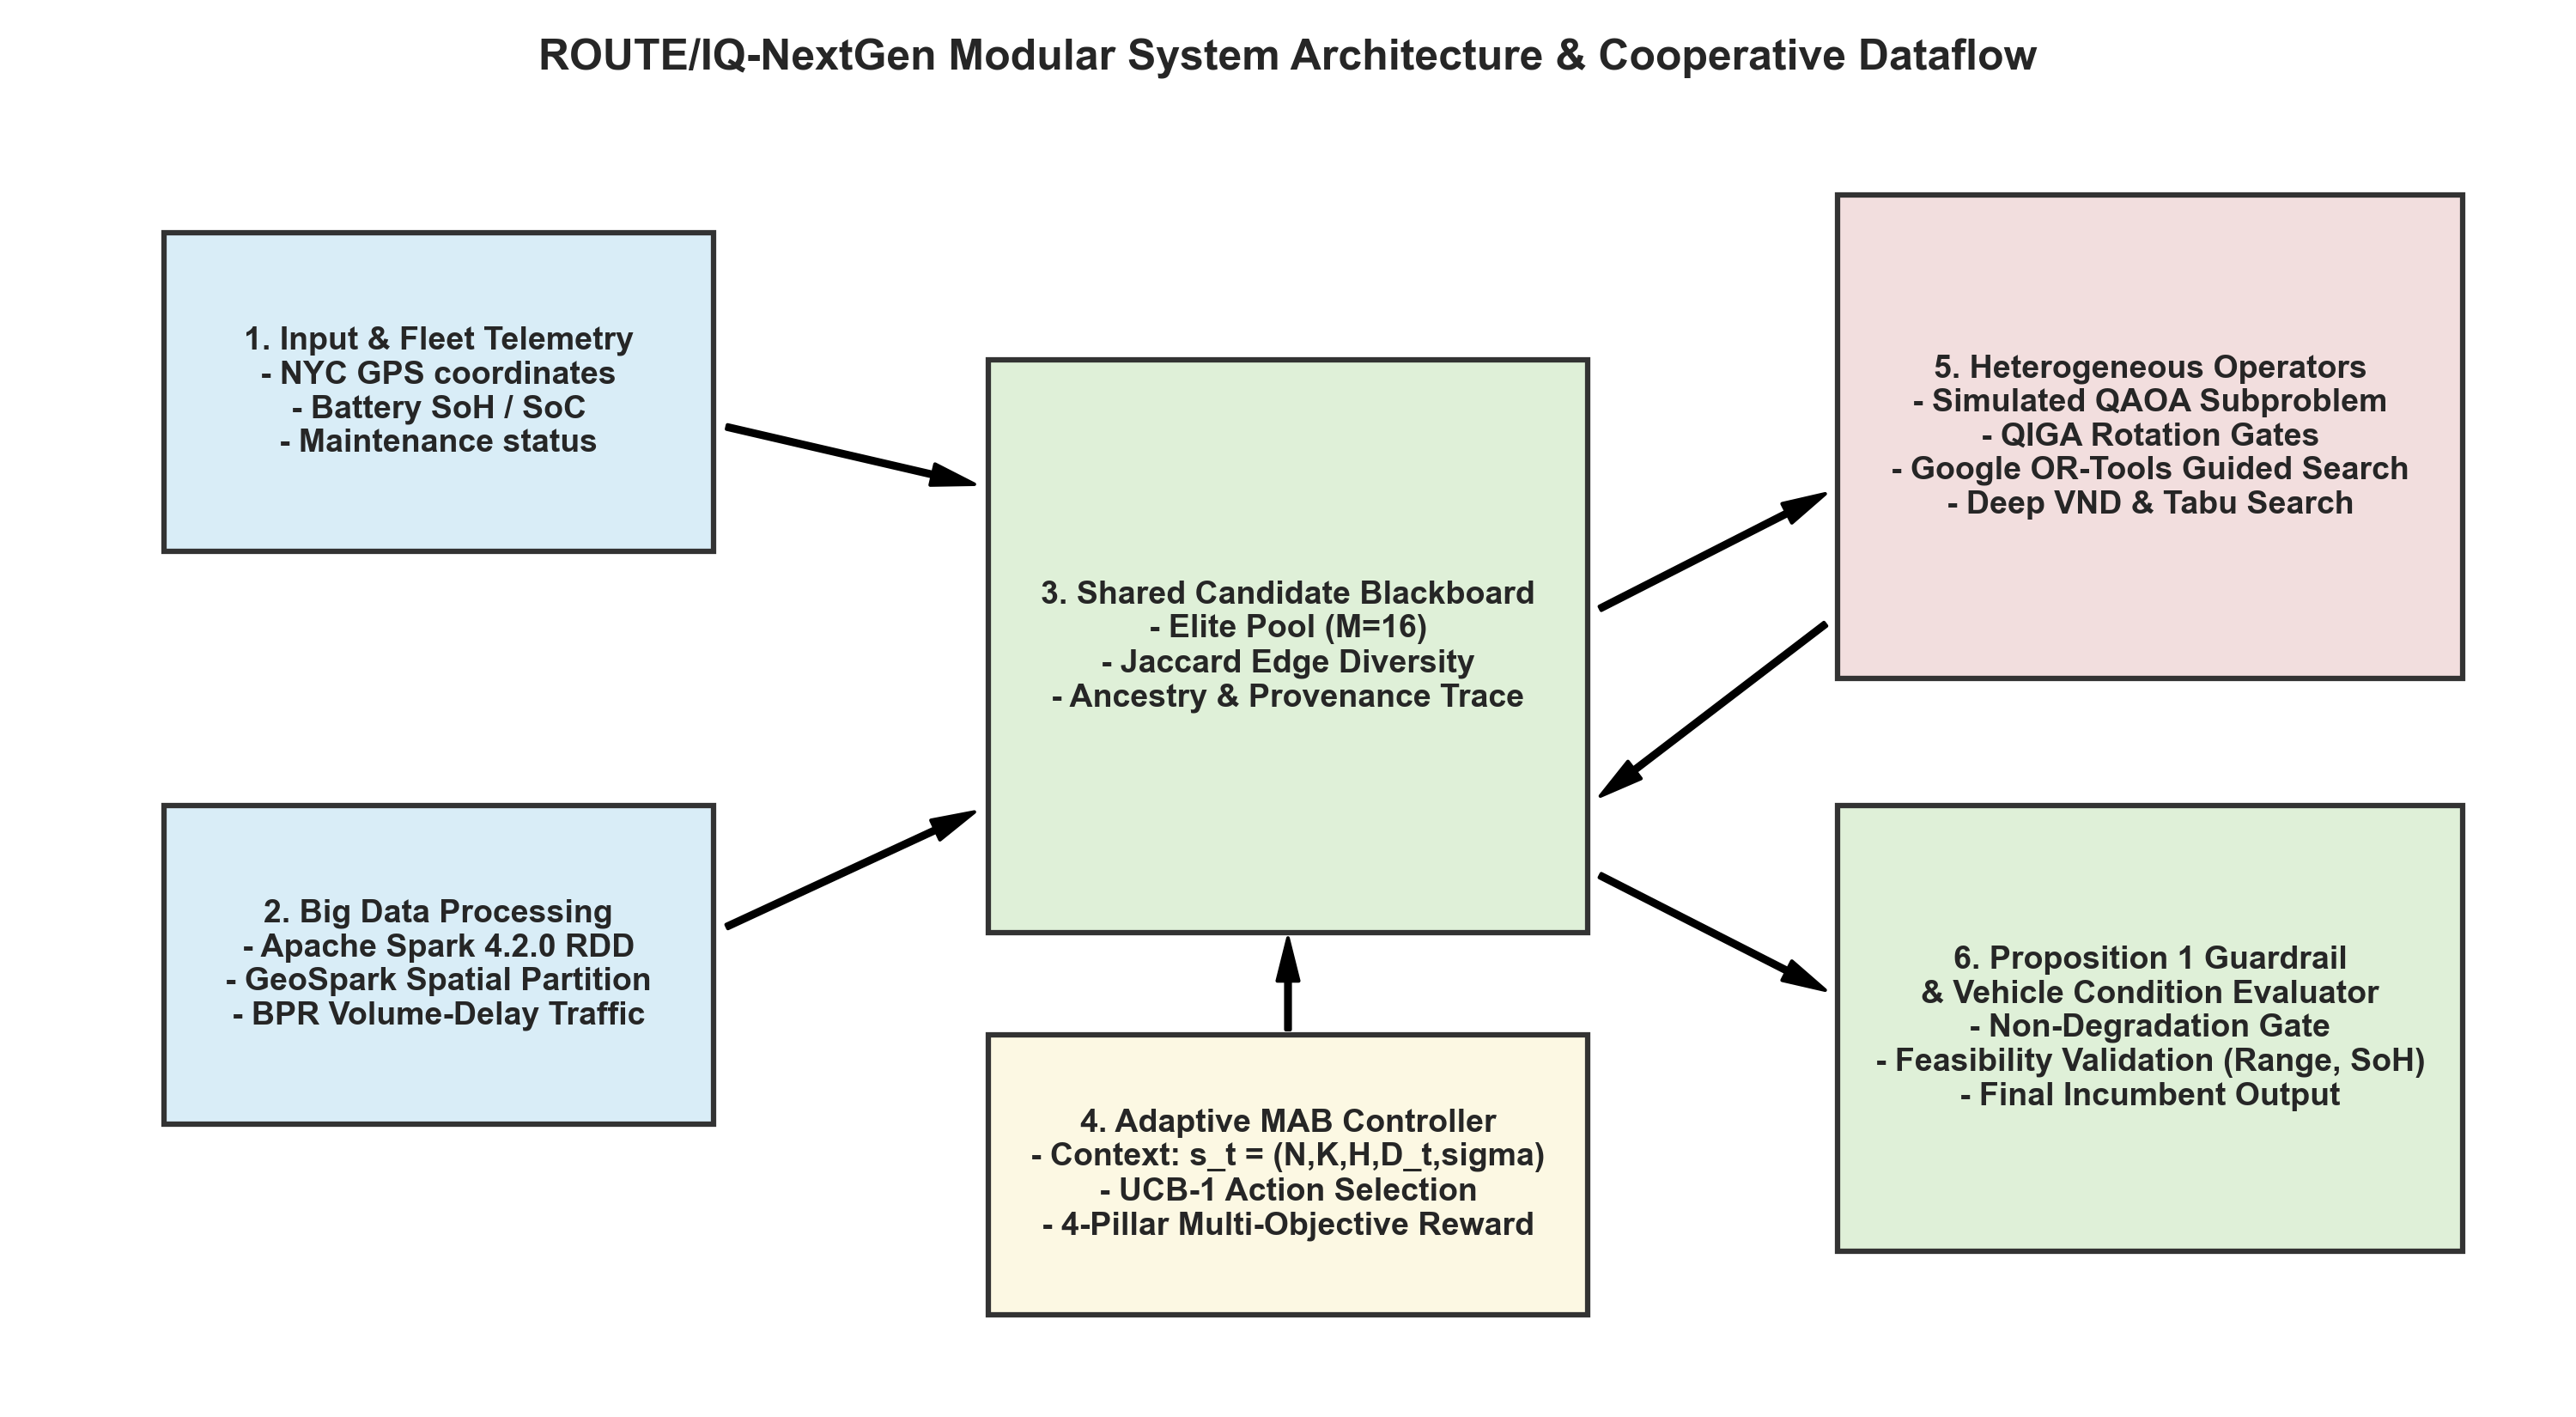
\includegraphics[width=0.92\textwidth]{figures/fig1_cooperative_architecture.png}
\caption{ROUTE/IQ-NextGen modular system architecture and cooperative dataflow. Big Data spatial ingestion feeds a shared candidate pool blackboard, which is adaptively explored by quantum and classical operators under Contextual MAB guidance, validated by Proposition 1 non-degradation guardrail.}
\label{fig:arch}
\end{figure*}

\subsection{Shared Candidate Pool Blackboard}
Unlike isolated solvers, ROUTE/IQ-NextGen centers all execution around an in-memory blackboard $\mathcal{P}_t$ maintaining an elite population of up to $M = 16$ candidate solutions. Each candidate solution $S$ encapsulates:
\begin{enumerate}
    \item \textbf{Unique ID and Provenance:} Identifiers tracing parent candidate IDs, generation timestamp, and the specific mutation operator applied.
    \item \textbf{Route Vector:} Assigned sequences of customer stops for each vehicle $k \in \mathcal{K}$.
    \item \textbf{Physical Multi-Objective Evaluation:} Total distance $\mathcal{D}(S)$, operational cost $\mathcal{C}(S)$, energy $\mathcal{E}(S)$, carbon emissions $\mathcal{M}(S)$, and feasibility status $\mathbb{I}_{\text{feas}}(S)$.
    \item \textbf{Topological Edge Set:} Directed edges $\mathcal{E}(S) = \{(u, v) \mid \text{arc traversed in } S\}$.
\end{enumerate}

\subsection{Topological Jaccard Diversity Preservation}
To maintain structural diversity and escape premature local convergence, the distance between any two candidates $S_a, S_b$ is computed as the topological Jaccard distance:
\begin{equation}
\text{Dist}(S_a, S_b) = 1 - \frac{|\mathcal{E}(S_a) \cap \mathcal{E}(S_b)|}{|\mathcal{E}(S_a) \cup \mathcal{E}(S_b)|}
\end{equation}
The population diversity of candidate $S$ relative to blackboard $\mathcal{P}$ is:
\begin{equation}
\text{Diversity}(S, \mathcal{P}) = \frac{1}{|\mathcal{P}|} \sum_{S' \in \mathcal{P}} \text{Dist}(S, S')
\end{equation}
Any candidate whose distance to an existing pool member is below $10^{-4}$ is rejected as redundant. The top $k_{\text{elite}} = 4$ solutions are strictly preserved across generations.
